\documentclass{scrreprt}
\usepackage[utf8]{inputenc}
\usepackage{lmodern}
\usepackage{listings}
\usepackage{underscore}
\usepackage{graphicx}
\usepackage[margin=0.5in]{geometry}
\usepackage[bookmarks=true]{hyperref}
\hypersetup{
    bookmarks=false,    % show bookmarks bar?
    colorlinks=true,       % false: boxed links; true: colored links
    linkcolor=blue,       % color of internal links
    citecolor=black,       % color of links to bibliography
    filecolor=black,        % color of file links
    linktoc=page            % only page is linked
}%
\def\myversion{1.0 }
\title{%
\flushleft
\rule{16cm}{5pt}\vskip1cm
\Huge{DESIGN SPECIFICATION}\\
for\\
Pok\'eSnowdown \\
\vspace{2cm}
\LARGE{Version \myversion\\}
\vspace{2cm}
Produced by Matthew Zang, Nicholas Shieh, Chirag Bharadwaj, Young Chan Kim\\
\vfill
\rule{16cm}{5pt}
}
\renewcommand\thesection{\arabic{section}}
\renewcommand\thesubsection{\thesection.\arabic{subsection}}

\date{}
\usepackage{hyperref}
\begin{document}
\newgeometry{left=3cm,bottom=0.1cm}
\maketitle
\tableofcontents
\restoregeometry
 
\section{System Description}
\subsection{Core Vision}

Our plan for A6 is to create a Pok\'emon Showdown spinoff using \texttt{OCaml} using key concepts presented in class (concurrency, mutability, functional programming) as well as integrating functions of \texttt{OCaml} not presented in class, including producing a suitable GUI and server to aid in development of the game. To set us apart from Pok\'emon Showdown, we are incorporating a single-player story mode in the form of a "Tournament mode", as well as allowing for full 1-Player, 2-Player, and No-Player functionality (by developing an intelligent bot that can fully play the game).

\subsection{Key Features}
We have the following incorporated in our following project.
\begin{enumerate}
	\item A fully functional GUI that allows the players to see the current state of the game. The GUI shows the current Pokemon in battle, the current statuses of the Pokemon, any stat modifications, etc... 
	\item All the current Pok\'emon are ncluded in the game. We have implemented 721 Pok\'emon over 400 moves, around 50 abilities, and around 6 items.
	\item Multiple game options. We have the following modes.
		\begin{itemize}
			\item For 1-Player, we incorporated three different modes. 
				\begin{enumerate}
					\item \textbf{Random Battles}: This is the same game mode as commonly found on Pok\'emon Showdown where teams are randomized. However, the player will be playing against the AI. 
					\item \textbf{Tournament mode}: This is the single player story mode. You battle Premade trainers with custom Pok\'emon sets. The story is that there is some Hunger Games activity, and Professor Oak is the captain who forces you to battle all the enemy trainers. As you beat trainers, you steal some of their Pok\'emon. Lastly, beat every trainer once and something special happens -- Professor Oak goes into the cave and you are allowed to battle him once. Win and you unlock a legendary Pok\'emon. Lose and you have to battle all the other trainers once more.
					\item \textbf{Preset Battles}: The player gets to create his own Pok\'emon team and play against AI that also use his unlocked Pok\'emon. 
				\end{enumerate}
			\item For 2-Player, we hope to have a two game modes.
				\begin{enumerate}
					\item \textbf{Random Battles}: Similar to One Player random battles, but against another player instead of an AI. 
					\item \textbf{Preset Battles}: Both players get to choose 6 Pok\'emon from the unlocked Pok\'emon before battling.
				\end{enumerate}
			\item Lastly, for No-Player, we hope to have a single game mode.
				\begin{enumerate}
					\item \textbf{SkyNet Battles}: Player watches the AI face each other with randomized Pok\'emon.
				\end{enumerate}
		\end{itemize}
	\item We provided a Pok\'emon team editor that allows a player to choose Pok\'emon and movesets. This team is saved and can be loaded up for future use. These teams will be used in the game modes described above.
	\item We wish to include a unique menu system and good GUI Animations.
	\item We included a simple interactive story mode/dialogue that will describe the underlying storyline in our Tournament mode. 
	\item We have included a very nice auto-saving feature that saves the game for you. 
	\item We have also included key-board input. During battle, the user must press SPACE BAR to proceed to the next text option. In addition, keyboard input is used to move the character during Tournament mode. 
\end{enumerate}

\subsection{Narrative Description}
	This game will be an upgraded version of Pok\'emon Showdown, suitable and to the scale for a small console video game. It will have the main aspects of Pok\'emon Showdown including random battles between two players, as well as premade team battles between two players and a fully functional Pok\'emon team editor. However, it will also include single player capabilities, such as random battling or premade battling against an AI. The AI must be able to battle effectively and use advanced Pok\'emon techniques in the battle. In addition to this, there will be a Tournament mode which is essentially a story mode. The player has to play against several bots before proceeding to the final boss. This means that bots should have different levels of intelligence in order for this game mode to be challenging. 
\section{Architecture}
	We produced a pipe and filter architecture. We were initially going to produce a client-server architecture with a game server keeping track of the current game state and updating the GUI will allowing clients (players) to send messages to the server to retrieve information and request actions; however, we realized that creating a server would make it hard to implement all the other features we wanted to implemented (since none of us knew what creating a server entailed). Instead of having a client-server architecture that allowed for two players to do concurrent battling, we realized that a pipelined architecture where each player would take turns choosing a move would work just as well. The input from the user will be passed along a pipeline and transforms the data into output. This is sufficient enough for the turn based Pok\'emon game. 
	
	However, in addition to the pipe and filter architecture (in relation to the game flow), we have some aspects of Shared Data Architecture. The Game and the GUI use the shared data architecture to communicate by reading and writing to the shared data. The C\&C diagram is provided below. The pipeline flow is shown from left to right, while the shared data architecture is shown extending downwards from Game Controller. 
	
	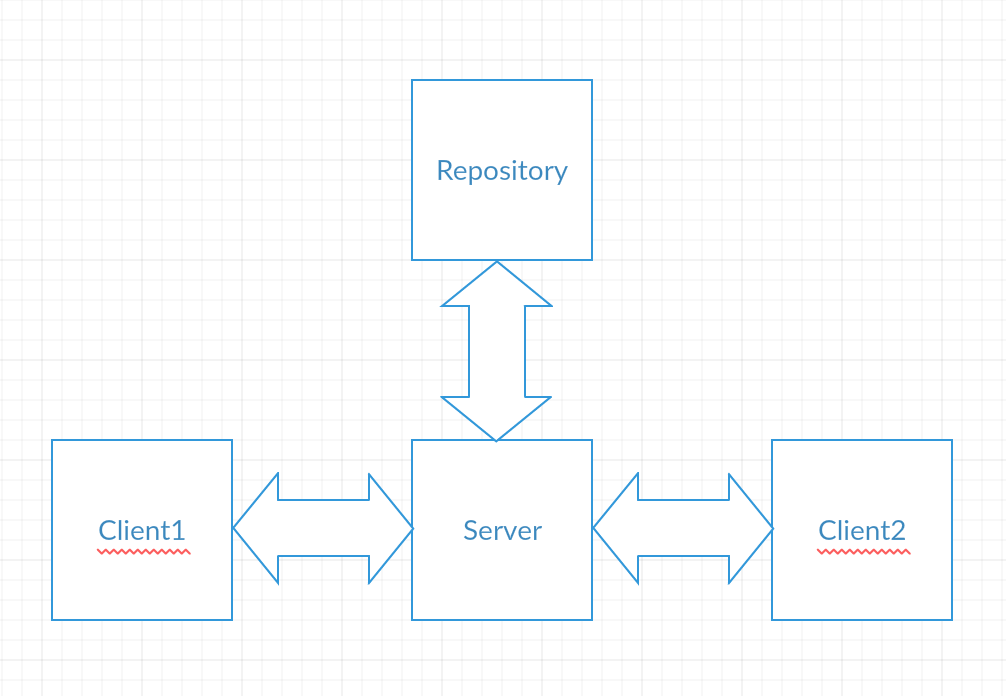
\includegraphics[scale=0.75]{C&C.png}

%TODO if you think of anything/want to upgrade MDD diagram
\section{System Design}
\subsection{Important Modules}

\begin{enumerate}
	\item \textbf{Game}: This is the game controller. It is mainly involved in handling the GUI and passing control to the battle controller when a battle occurs/is set up.
	\item \textbf{Gui}: The Gui is used to diplay the current state of the game. There are two main phases in the Gui, the menu screens and the battle scenes. The Gui will either communicate with the game controller when the menu screens are being displayed or communicate with the battle controller when a battle is occuring.
	\item \textbf{Info}: The Info module contains all the data types that are needed/shared between the module. It essentially contains everything the other modules need to use to communicate with one another and helps in avoiding circular dependencies. All data types needed for the game will be declared here.
	\item \textbf{BattleController}: This battle controller module is called by the game controller when a battle is taking place. During this time, the battle controller handles all the game mechanics and updates the Gui. The game controller waits for the battle to end before resuming control.
	\item \textbf{Pok\'emon}: This module is involved in loading the data from the json files and getting Pok\'emon data. It is responsible for turning the Json data into a Pok\'emon. For example, functions in this method will be called to convert a string containing the name of the Pok\'emon to some value of type Pok\'emon (defined in the Info module). 
	\item \textbf{AI}: This module will be involved in the artificial intelligence aspect of our game, where we will handle the bots playing the game automatically for the SkyNet Battles. For instance, this module should contain functions that will allow a bot to intelligently select moves to maximize damage to the opposing bot while minimizing its own damage and moves used. 
	\item \textbf{Tournament}: This contains all the tournament data. It has the opponent's in tournament mode, the map of the tournament mode, the different trainer classes, and it makes calls to Save after a battle has been won.
	\item \textbf{Save}: This module makes all the save calls. While Pok\'emon turns json to Pok\'emon, Save turns json to a Pok\'emon. 
\end{enumerate}

\subsection{Module Dependency Diagram}
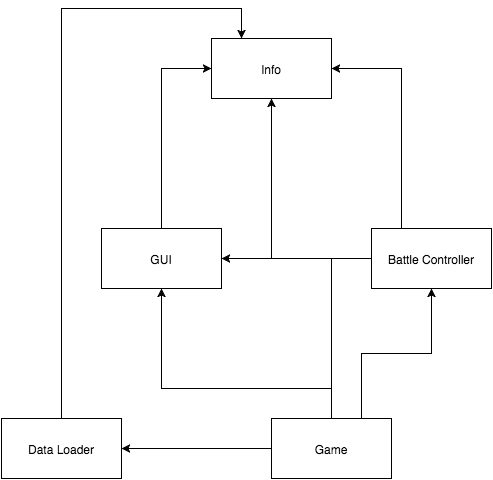
\includegraphics[scale=0.75]{MDD.png}

\section{Data}
%TODO Fill in internal data
\subsection{Internal Data}
We have all the json files to represent all the Pok\'emon, moves, abilities, etc... Since json files aren't readily available online with all the Pok\'emon data, we wrote \texttt{Python} scripts to fetch the data from databases and convert them to a json format. To load the data, we used the \texttt{Yojson} module, similar to how we used it in A2. In addition, we have many jpgs and gifs that represent the Pok\'emon. We used many of the resources on Smogon and Bulbapedia to obtain information.

%TODO Fill in communication
\subsection{Communication}
In order to let the GUI communicate with the Game without the use of a server, we came up with a method of communication through Ivar references. When Game initializes the GUI, we will make Game pass in as an argument an Ivar reference. Game and GUI will communicate by emptying and filling the Ivar. When Game is ready to handle another input, Game will reset the Ivar by creating a new one. GUI will then fill in the Ivar upon receiving some input. Thus, Game and GUI will be able to communicate without creating any circular dependency among modules. The Ivar will be filled with some value that is of type \texttt{game\_state} defined in the Info module. 

%TODO Fill in data structures
\subsection{Data Structures}
We held all the Pok\'emon data in Json files. We did have many Variants to hold the secondary effects of the game. While Battle Controller did the damage calculation and secondary effect dependencies, it used variants to hold all the different secondary effects that happened during the move processing. It then sends this variant to the GUI which unpacks it nicely as a message in the battle to the user. In addition, these variants are also decomposed to get the right attack animation. The Pok\'emon themselves are stored as mutable records. The trainers are stored as records with a field for the current Pok\'emon in battle, a field for a list of alive Pok\'emon and a field for a list of dead Pok\'emon. 

%TODO See if you can expand
\section{External Dependencies}
We used  \texttt{Lablgtk2} to create the GUI and \texttt{Yojson} to parse json files. The json data will primarily be collected from \url{https://github.com/veekun/pokedex/tree/master/pokedex/data/csv} using \texttt{Python}.

%TODO Fill in testing plan 
\section{Testing Plan}

\textbf{Previous Testing Plan:}

Our testing plan will mainly consist of debugging and verifying individual functions through a combination of black-box and white-box testing for each module, as well as regression tests to ensure any changes to some aspect of our program does not break an existing functionality that was previously verified. These test cases will be mostly randomized and automated, and testing will take place during and after the implementation process. Of course, once we are finished with the implementation and modular testing, we will also test the overall gameplay by playing the game many times and letting some of our friends outside of the course to play the game to assure that the game can be played without issues and also receive useful feedback. If we have time, we may even formally verify the correctness of some of our functions.

\textbf{Our Testing Plan: }

Our testing plan was primarily done during the hard coding phase. We divided our project into three main phases -- data preparation, gui creation, and hard coding. Data Preparation was necessary to get all the data of the Pok\'emon. This was obtained by downloading csv files and parsing them into JSON format using Python. No testing had to be done in this phase.

The GUI Creation phase was done next. It was simply the creation of the GUI and creating all the menus/simple game animations. This was done with peer review testing. We made sure all code was functional before it was pushed. There are no big bugs in the GUI. However, there are times when the Game is stuck in the Loading Screen. This is easily fixed by closing and rerunning the game. 

After GUI Creation, we had to do the hard coding. We hard coded all the different moves/abilities. There are no known bugs in the moves/abilities. This was because we thoroughly tested every move/secondary effect before allowing it to be in the game. 

\section{Division of Labor} 

\textbf{Matthew Zang:}

He primarily did the GUI, managing the team, getting the json data, and setting up the project. He also assigned tasks to everyone. He made the menu for the GUI, the loading screens, battle animations, and designed the overall Game Logic. He also wrote the Poke Editor and the main menu screens.

\textbf{Nick Shieh:}

He was primarily in charge of hard coding the moves. He helped code the majority of the moves and making sure the interactions were clear. Nick was also in charge of coding the AI for the game. He and Young made two different difficulty levels for the AI, a simple one and a more complex one. However, only the complex one was included as an opponent in the game, as the simpler one served to be way too naive to even people that have never played Pok\'emon before. 

\textbf{Chirag Bhardawaj:} 

He was in charge of testing, code verification, and getting the game animations and images. He also made the Tournament mode of our game, the tile-maps, and retrieved the sprites for the opponents. He also coded the Save File handler, which was vital for the saved state of our game. Additionally, he was in charge of the graphics design of our game. 

\textbf{Young Chan Kim:} 
 
He was also in charge of hard coding the moves. He helped code the majority of the moves and handling the GUI interactions for the Pokemon moves. He also made a major contribution to the AI of the game. In addition, he also was primarily in charge of coding the abilties and items that were used throughout the game. He also designed the formats for the Data structures, such as the records for the Pok\'emon, records for the moves, variants for elements and secondary effects, etc.
 
% add other chapters and sections to suit
\end{document}